\lhead{Background}
The problem statement is defined in the previous chapter, along with the outline of this thesis. As described in the introduction, the focal point is oversampling imbalanced data to help in classification problems. The first step is to describe popular methods when dealing with imbalanced data, before moving to the proposed model.

\section{Dealing with imbalance}
There are three popular methods for imbalanced data that will be discussed here: cost-sensitive learning, data level preprocessing methods and algorithm-level approaches. Data level preprocessing includes oversampling and undersampling. These methods handle imbalanced data during three different phases in model training. Algorithm-level approaches focus on modifying the classifier learning procedure without altering the data itself~\cite{Fernandez2018LearningSets}. This process requires an understanding of the classifier's mechanics, which leads to a bias towards the majority class. As this topic is not the focal point of the thesis, and since there are many classifiers, each having alterations, this topic will be limited to decision trees.

The first method depends on selecting the right algorithm and understanding its limitations in order to improve it. Decision tree classifiers are simple and efficient, and offer an interpretable solution~\cite{Safavian1991AMethodology}. A complex decision is split into a union of several smaller decisions, leading to the shape of a tree. Due to their simplicity, it is also easy to alter them from the algorithm-level approach. To change the behaviour of the model, one only needs to change the split function responsible for the decisions. Changing this key component is therefore the most straightforward approach possible. 

Secondly, cost-sensitive learning is an aspect of an algorithm-level approach, but it does not alter the core algorithm itself. Instead, it introduces a missclassification cost which penalizes mistakes during classifier training. Concerning imbalanced learning this means that missclassifying the minority class is penalized during learning. The effect of imbalanced data on cost-sensitive learning has been studied~\cite{Liu2006TheStudy}, claiming that cost-sensitive classifiers still prefer a natural class distribution. In other words, highly imbalanced data needs to be balanced before applying cost-sensitive learning.

This leads to the final approach: data level preprocessing. This method involves the balancing of class distribution and can be done in three ways~\cite{Batista2004AData}
\begin{itemize}
    \item \textbf{Undersampling:} creating a subset of the original dataset by removing samples usually (from the majority class).
    \item \textbf{Oversampling:} creating a superset of the original dataset by replicating samples or creating new ones.
    \item \textbf{Hybrid methods:} Involve a combination of the undersampling and oversampling.
\end{itemize}
The most straightforward procedure is random undersampling or random oversampling. As the name suggests, it does not consider the relevance of any of the data samples, but it chooses random data samples and copies them. Random undersampling has the drawback that it potentially removes useful data, leading to worse performance. Alternatively, Random oversampling can increase the risk of overfitting, as the method makes exact copies of existing samples~\cite{Fernandez2018LearningSets}. Both undersampling and oversampling have been studied and many methods have been proposed. This thesis focuses on oversampling, specifically SMOTE-based oversamplers.

\section{SMOTE algorithm}
SMOTE is an acronym for Synthetic Minority Oversampling TEchnique. The method was first introduced by Chawla et al.~\cite{Chawla2002SMOTE:Technique} in 2002. The main idea is to introduce new, synthetic samples to the dataset to make it balanced. These samples are created by interpolation between samples of the minority class. 

\begin{figure}
    \centering
    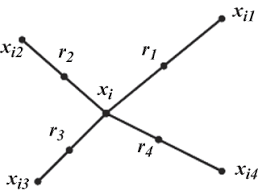
\includegraphics[width=.4\textwidth]{Thesis/Figures/SMOTE_alg.png}
    \caption{An illustration of how to create synthetic data samples using the SMOTE algorithm~\cite{Fernandez2018LearningSets}.}
    \label{fig:SMOTE}
\end{figure}

An example of the SMOTE algorithm works is given in figure~\ref{fig:SMOTE}. First, a sample $x_i$ is taken from the minority class. Then, using a distance metric (i.e. Euclidean distance), $k$ nearest neighbours are selected, points $x_{i1}$ to $x_{i4}$. Finally, these points are randomly interpolated to create new instances labelled as $r_1$ to $r_4$. This process is repeated until the desired ratio between the majority and the minority classes is achieved. 

\section{SMOTE extensions}
SMOTE is now widely known and easy to implement in Python, due to its inclusion in the Imbalanced-learn package~\cite{Lemaitre2017Imbalanced-learn:Learning}. Since 2002, many variations of SMOTE were introduced, changing parts of the algorithm to improve its performance in classification. It is uncertain what the total amount of variants is, but a study by Kovacs et al. from 2019 included 85 SMOTE-variants~\cite{Kovacs2019AnDatasets}. While the number of variations is high, the main principle stays the same: SMOTE relies on a k-nearest neighbour algorithm. One can see that this works for samples in a continuous feature space. However, it is difficult to measure distance between two features that are categorical. These problems are often the reason why SMOTE-variants are introduced. Along with Chawla et al.'s original SMOTE algorithm, SMOTE-NC was also introduced~\cite{Chawla2002SMOTE:Technique}. NC stands for Nominal Continuous, and alters the distance metric to account for categorical features. Consider two features with both numerical and categorical samples
\begin{align}
    F_1 = [1,2,3,A,B,C]  \\
    F_2 = [5,6,7,A,D,E]
\end{align}
For the continuous features, the Euclidean distance can be easily calculated. If the nominal features differ between samples, then the median of standard deviations of all continuous features for the minority class is included. In the case of our two features, the Euclidean distance is calculated as
\begin{align}
    d_{Eucl} = \sqrt{[(5-1)^2 + (6-2)^2 + (7-3)^2 + Med^2 + Med^2]}
\end{align}
The synthetic samples are then generated similarly to SMOTE.

Another example is Borderline-SMOTE, which synthesizes minority samples near the decision boundary~\cite{Han2005Borderline-SMOTE:Learning}. This algorithm also considers the majority samples surrounding a minority sample. Suppose more majority samples than minority samples surround a minority sample. In that case, it is marked as easily misclassified and added to a special set $D$. Once all minority samples are considered, the samples from $D$ are then oversampled in the same way as in regular SMOTE.

Another SMOTE-based oversampler is ADASYN, an acronym for ADAptive SYNthetic sampling approach~\cite{He2008ADASYN:Learning}. ADASYN introduces a new learning constraint, using the weighted distribution for different minority samples according to their difficulty in learning. More samples will be synthesized for samples that are harder to learn. Similar to Borderline-SMOTE, a sample surrounded by majority samples is considered harder to learn. However, ADASYN uses a density distribution for all minority samples to decide where to synthesize new samples.

\begin{figure}
  \begin{subfigure}[t]{.5\textwidth}
    \centering
    \includesvg[width=\linewidth]{../Plots/Dummy/PC_Plot_standard.svg}
    \caption{Imbalanced dataset with no oversampling}
  \end{subfigure}
  \hfill
  \begin{subfigure}[t]{.5\textwidth}
    \centering
    \includesvg[width=\linewidth]{../Plots/Dummy/PC_Plot_SMOTE.svg}
    \caption{1:1 oversampling using SMOTE}
  \end{subfigure}

  \medskip

  \begin{subfigure}[t]{.5\textwidth}
    \centering
    \includesvg[width=\linewidth]{../Plots/Dummy/PC_Plot_BorderlineSMOTE.svg}
    \caption{1:1 oversampling using BorderlineSMOTE}
  \end{subfigure}
  \hfill
  \begin{subfigure}[t]{.5\textwidth}
    \centering
    \includesvg[width=\linewidth]{../Plots/Dummy/PC_Plot_ADASYN.svg}
    \caption{1:1 oversampling using ADASYN}
  \end{subfigure}
\caption{PCA plots for a dummy imbalanced dataset. Subfigure b-d show a 1:1 oversampling ratio using different oversamplers.}
\label{fig:oversampling}
\end{figure}

To illustrate this, a dummy dataset was created with a 95:1 imbalance ratio. Figure~\ref{fig:oversampling} shows the PCA plots of the original dataset, as well as the oversampled version using SMOTE, BorderlineSMOTE and ADASYN. SMOTE uses all available samples in the minority set to generate new samples, creating line segments spread out over the entire feature space. This is not as prevalent in BorderlineSMOTE and ADASYN, as they focus on samples which are difficult to learn. As a result, the concentration of new samples is higher when they are closer to the majority set. Both Adasyn and BorderlineSMOTE generate new samples in different locations, altering the result of the PCA plot. The new distribution of minority samples affects the classifier's learning process, which in turn affects the metric scores. The key in oversampling is to generate new samples which aid the classifier's learning process, in order to identify more minority samples.

\section{Generative Adversarial Networks}
SMOTE algorithms are not the only way of synthesizing data. In 2014, Goodfellow et al. introduced a novel way of generating data using a Generative Adversarial Network~\cite{Goodfellow2014GenerativeNets}. A GAN makes use of two contesting neural networks, one of which is a generative model $G$ which captures the data's distribution and is able to produce new samples. Simultaneously a discriminative model $D$ estimates if a generated sample comes from the training data instead of $G$\footnote{Detailed description of the architecture of GANs are omitted in this thesis as it is not relevant to Synthsonic}. This approach is now used for synthesizing video and images which are indistinguishable from their real counterparts. This led to GAN adaptations such as MedGAN~\cite{Armanious2018MedGAN:GANs}, aiding medical image analysis and image translation, and VeeGAN~\cite{Srivastava2017VEEGAN:Learning}. The latter emphasizes on the training method which could replicate the distribution of the dataset more accurately.